\section{3D Results}
\label{sec:3d_results}

In previous sections, we showed that changing the streaming order can significantly reduce error. For example,
adaptive RMSE optimized stream outperforms any fixed ordering stream, such as by level,
by bit plane, or by wavelet norm. We now validate those result on the full 3D datasets.
Since, the data sets are much larger, for
practical reason we had increase the group size from $4^2$ to $16^3$.

We start with reproducing the experiment comparing streaming the data \emph{by level}, \emph{by bit plane},
and \emph{by wavelet norm} (\Cref{fig:motivation-3d-rmse}). In 2D experiments, all data set exhibited the by level stream
being the worst, then by bit plane, and the best was by wavelet norm (REF). The 3D results are different as
the by level and by bit plane orders cross. The cause is that the by bit plane stream reads one bit plane for whole
dataset, but many of those will be zero and thus not contribute to the error reduction (TODO SLZ). In contrast, the by
level stream will read low subbands first and in most cases reduced the error as it is common that most energy is stored in
the these subbands.

\begin{figure}
  \centering
	\subcaptionbox{Boiler}
        {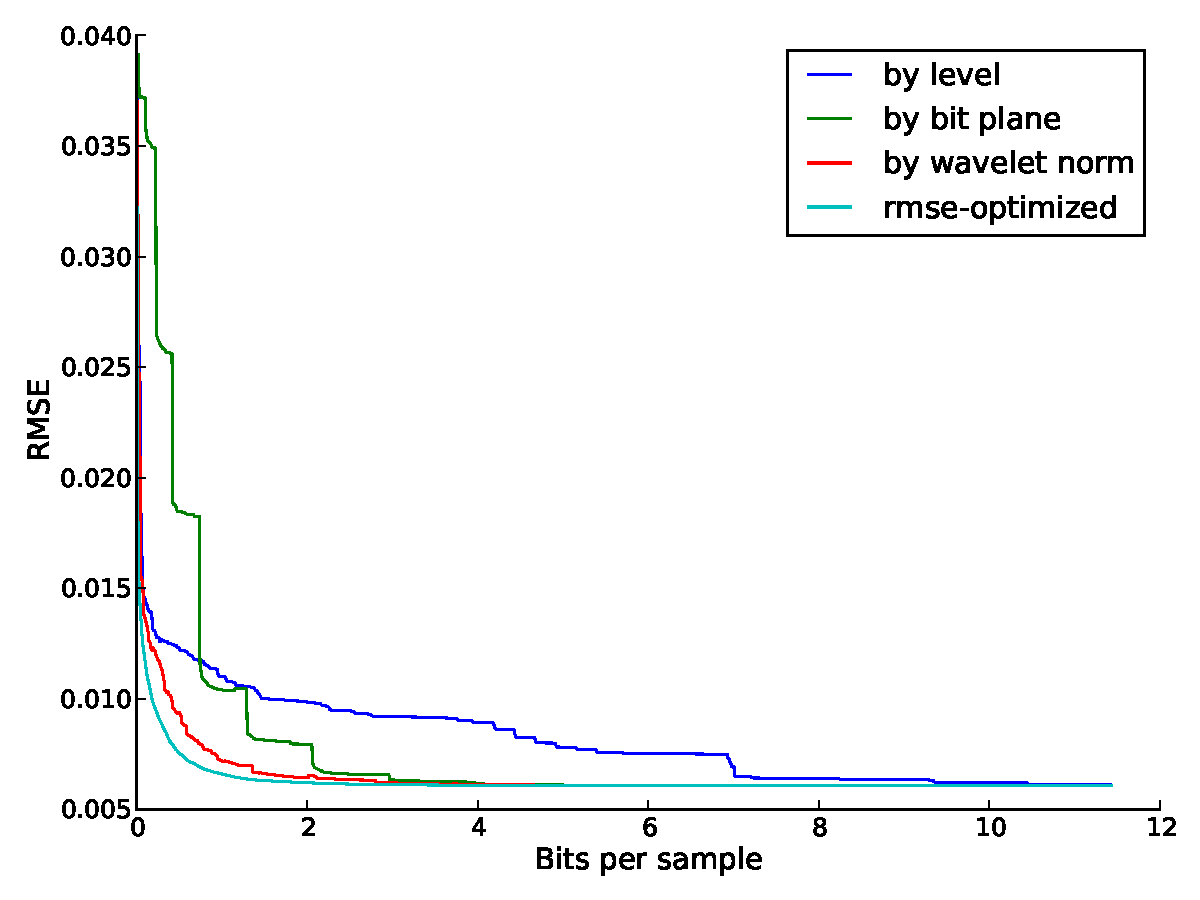
\includegraphics[width=0.48\linewidth]{img/motivation-3d/rmse-boiler.pdf}}
	\subcaptionbox{Diffusivity}
 	{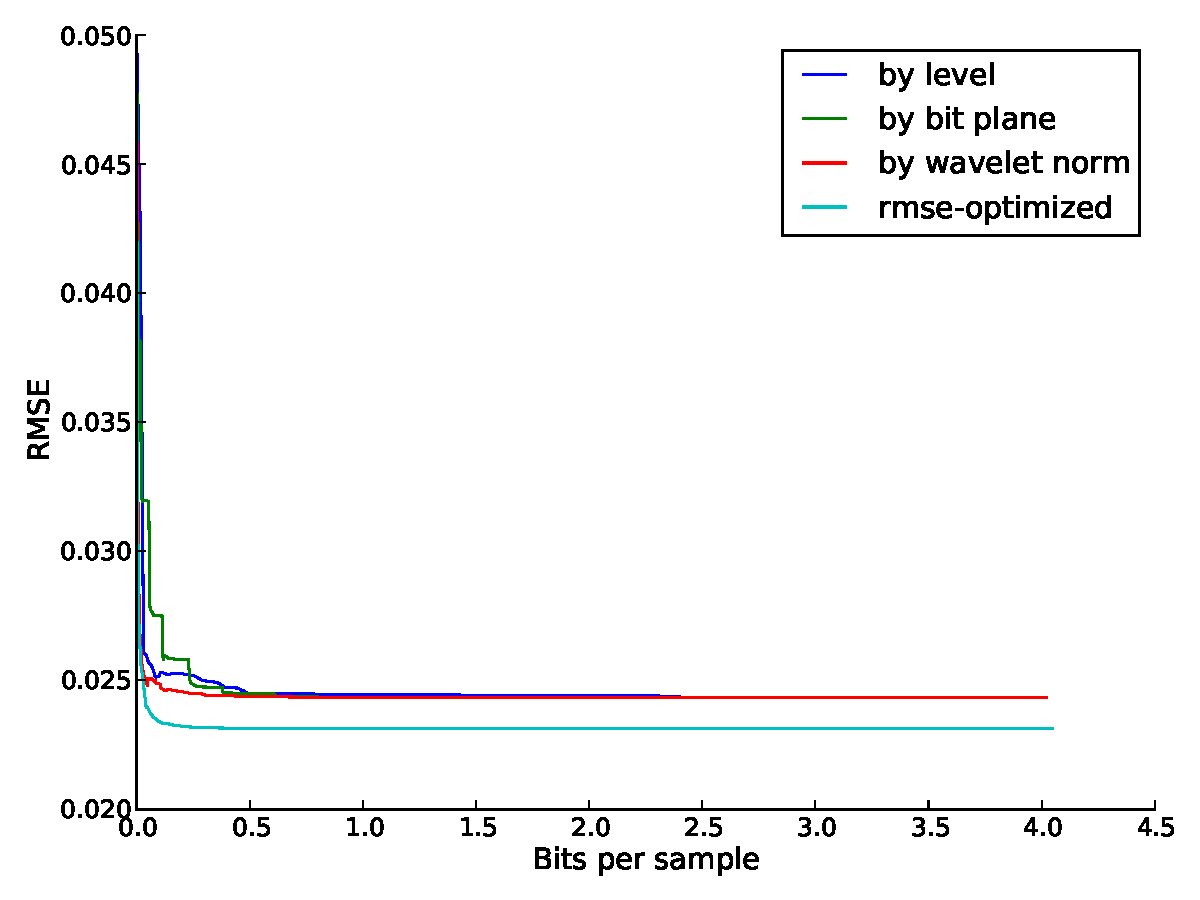
\includegraphics[width=0.48\linewidth]{img/motivation-3d/rmse-diffusivity.pdf}}
	\subcaptionbox{Turbulence}
 	{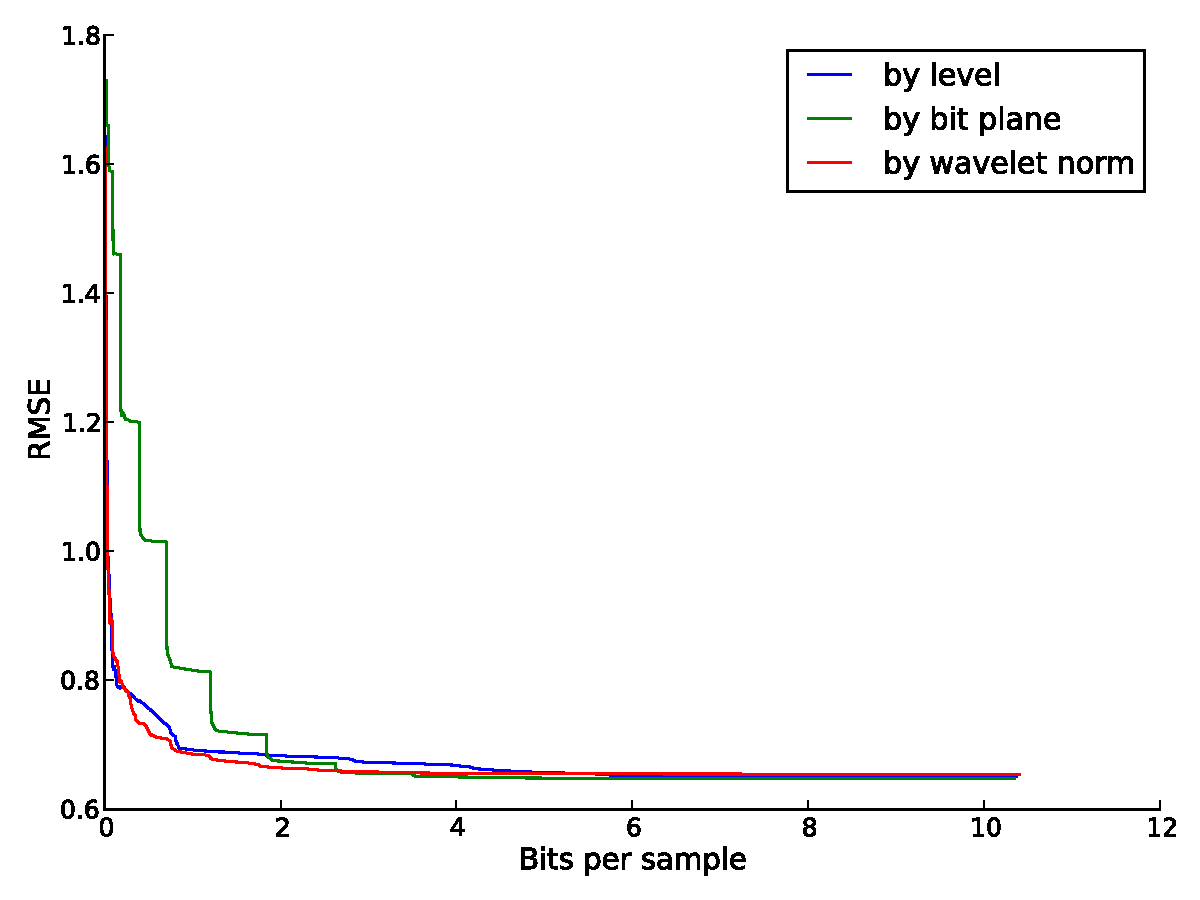
\includegraphics[width=0.48\linewidth]{img/motivation-3d/rmse-turbulence.pdf}}
	\subcaptionbox{Velocity-z}
 	{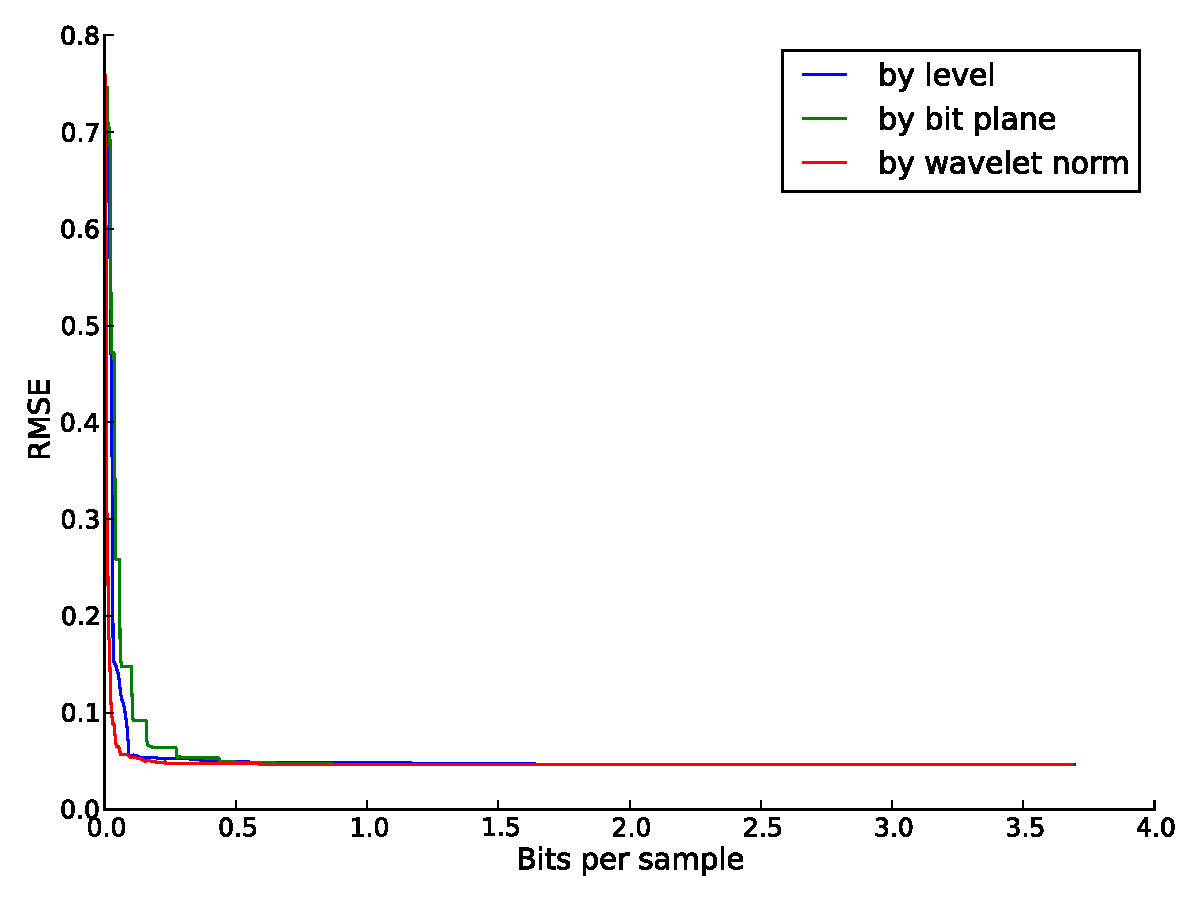
\includegraphics[width=0.48\linewidth]{img/motivation-3d/rmse-velocityz.pdf}}
 	\caption{Root-mean-square error for 3D datasets of reconstructed functions using the three data-agnostic streams
 	defined in Section \ref{sec:motivation} and the data dependant greedy scheme. Lower is better.
        The streams are truncated to highlight
 	the differences, without omitting important information. \pavol{explain why by level and by bit plane cross}}
 	\label{fig:motivation-3d-rmse}
\end{figure}


\begin{figure}
  \centering
	\subcaptionbox{Boiler}
        {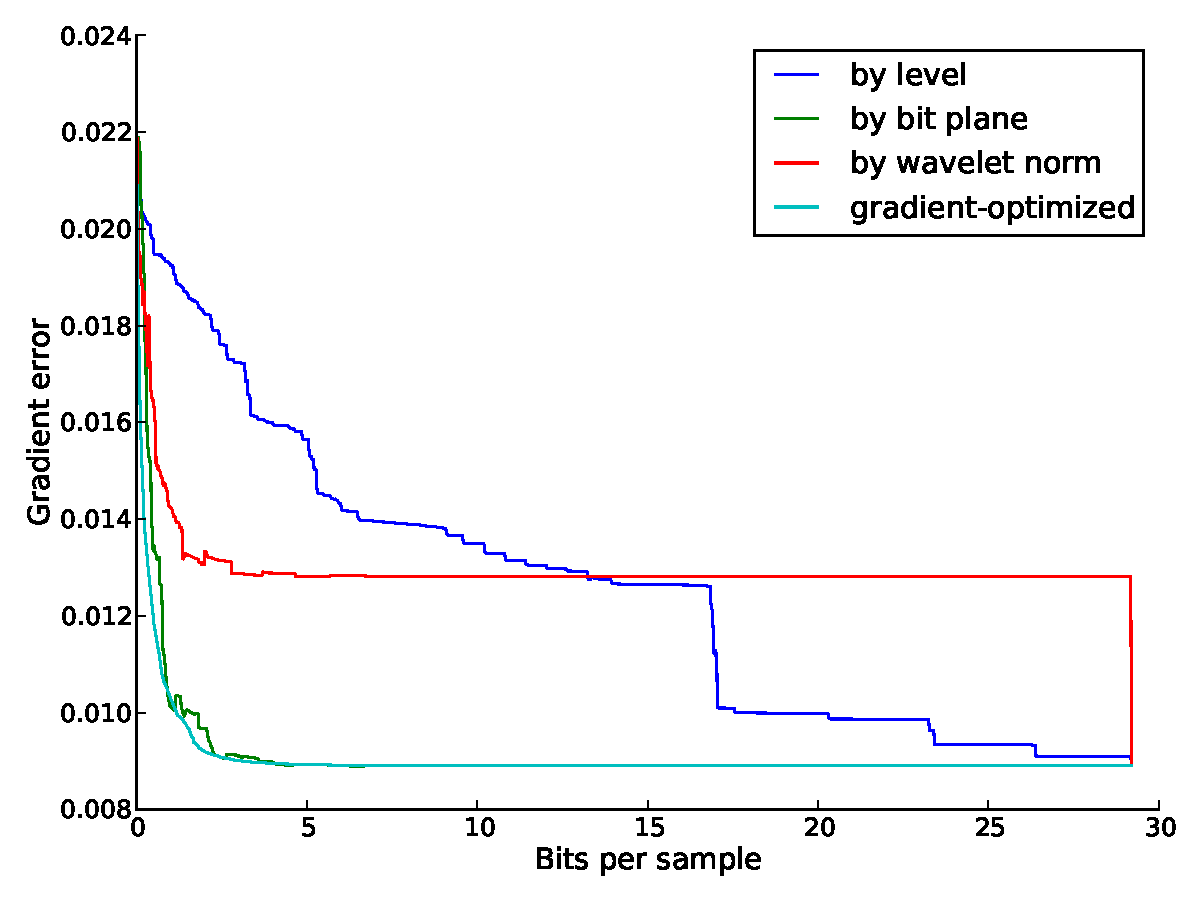
\includegraphics[width=0.48\linewidth]{img/motivation-3d/gradient-boiler.pdf}}
	\subcaptionbox{Diffusivity}
 	{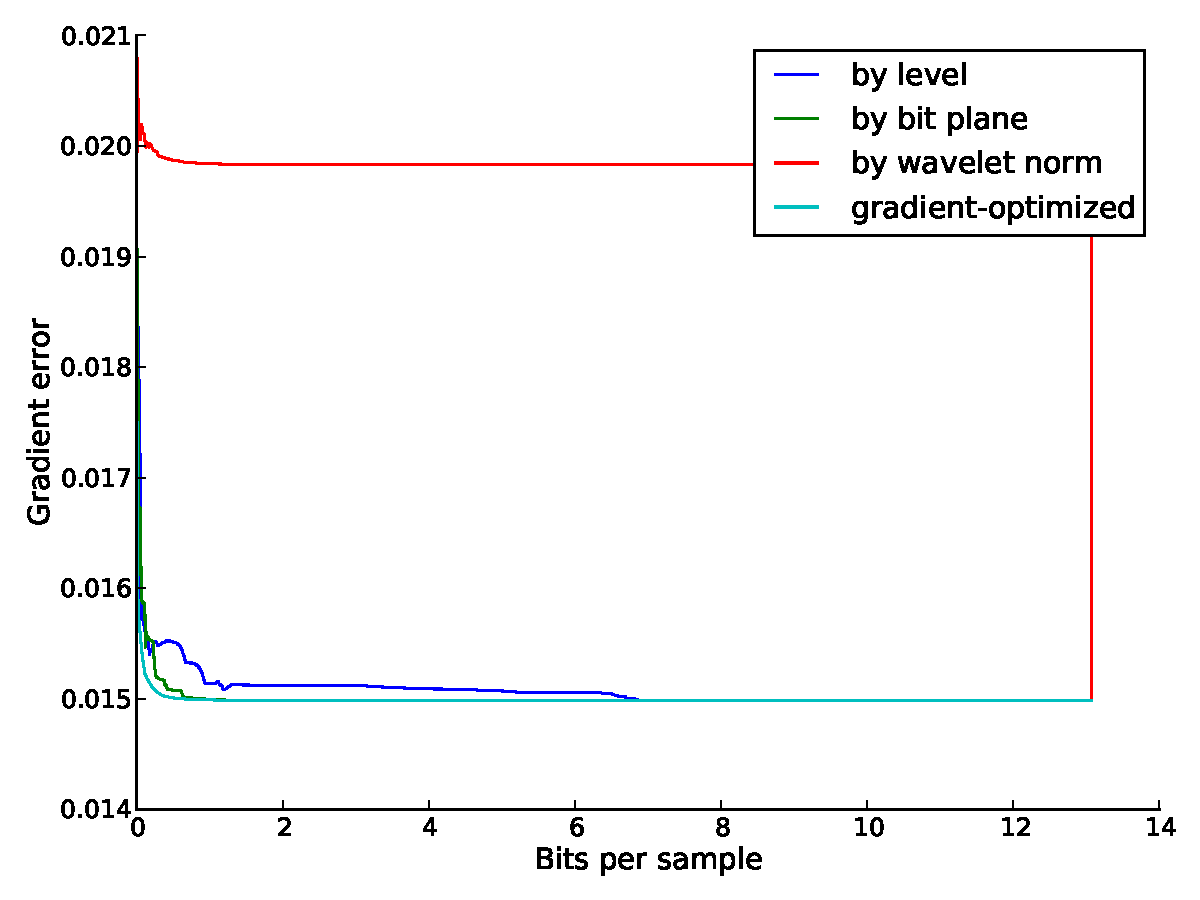
\includegraphics[width=0.48\linewidth]{img/motivation-3d/gradient-diffusivity.pdf}}
	\subcaptionbox{Turbulence}
 	{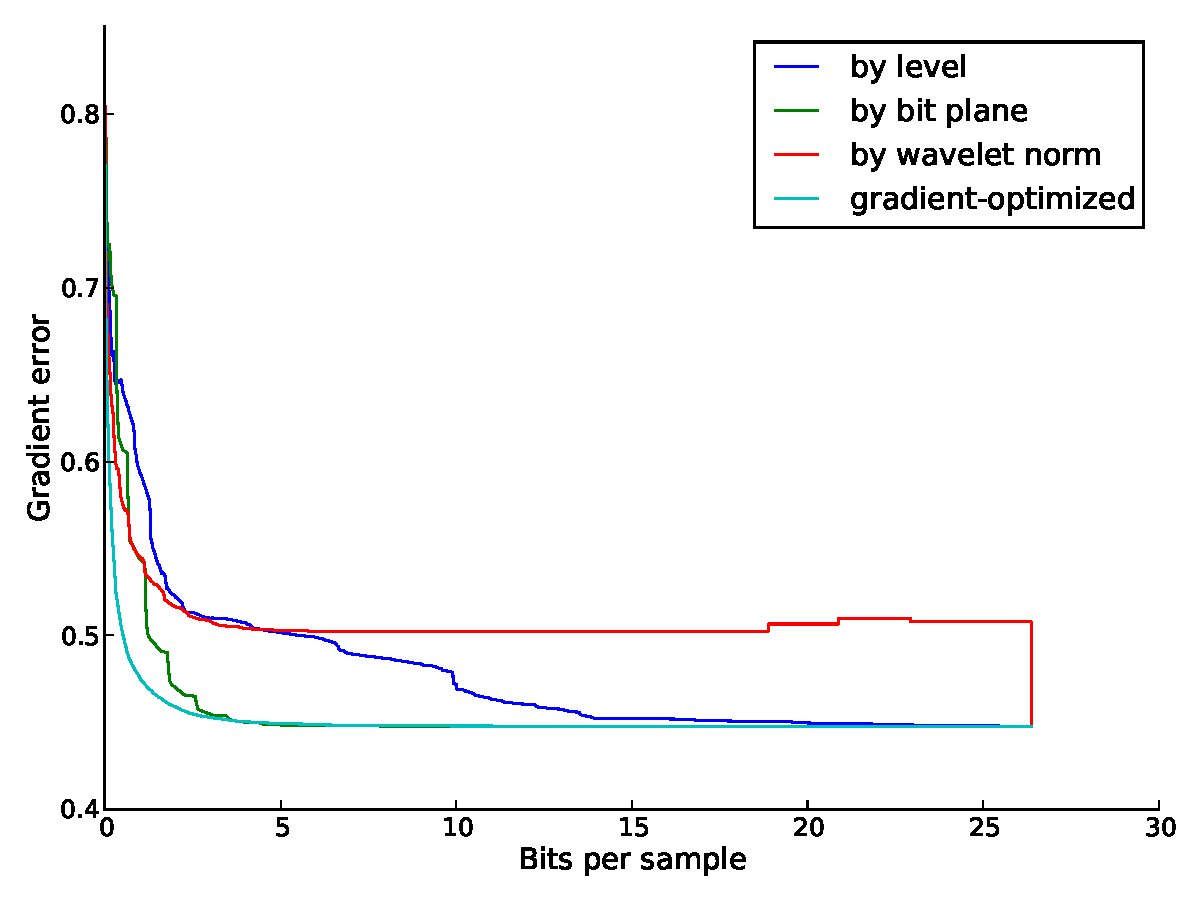
\includegraphics[width=0.48\linewidth]{img/motivation-3d/gradient-turbulence.pdf}}
	\subcaptionbox{Velocity-z}
 	{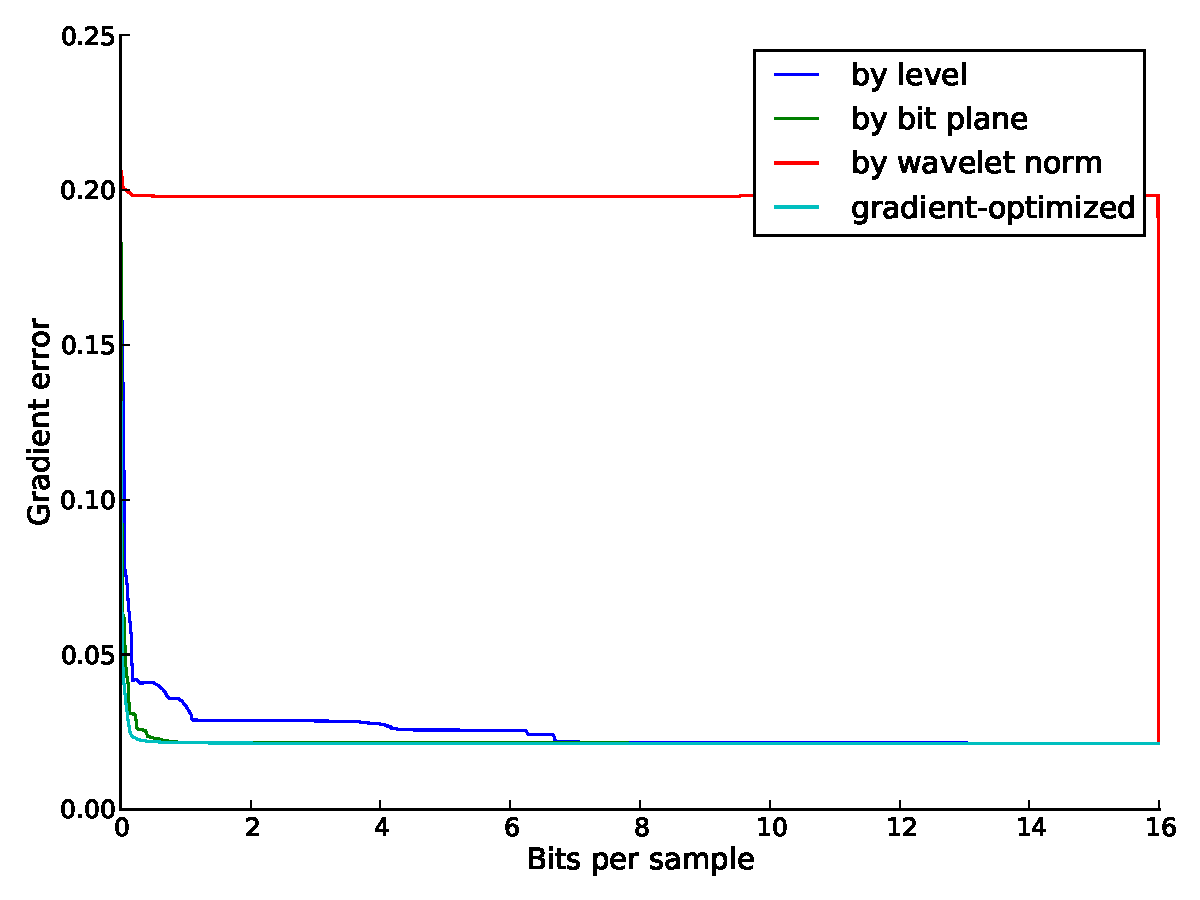
\includegraphics[width=0.48\linewidth]{img/motivation-3d/gradient-velocityz.pdf}}
 	\caption{Gradient error (3-point stencil) of reconstructed functions for 3D data sets using the three data-agnostic streams
 	defined in Section \ref{sec:motivation} and the data dependant greedy scheme. Lower is better.
        The streams are truncated to highlight
 	the differences, without omitting important information.}
 	\label{fig:motivation-3d-gradient}
\end{figure}

% commented out because the pdf files are missing
% \begin{figure}
%   \centering
% 	\subcaptionbox{Boiler}
%         {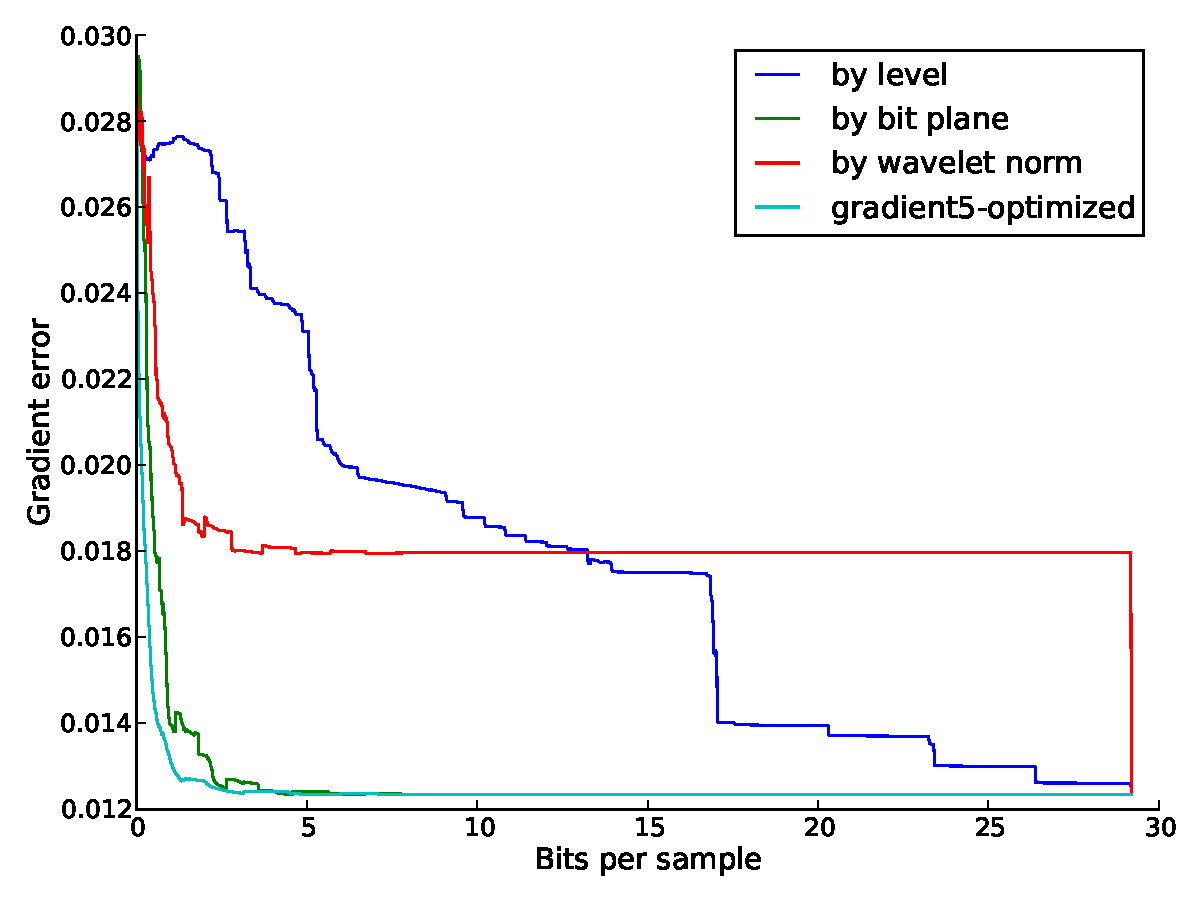
\includegraphics[width=0.48\linewidth]{img/motivation-3d/gradient5-boiler.pdf}}
% 	\subcaptionbox{Diffusivity}
%  	{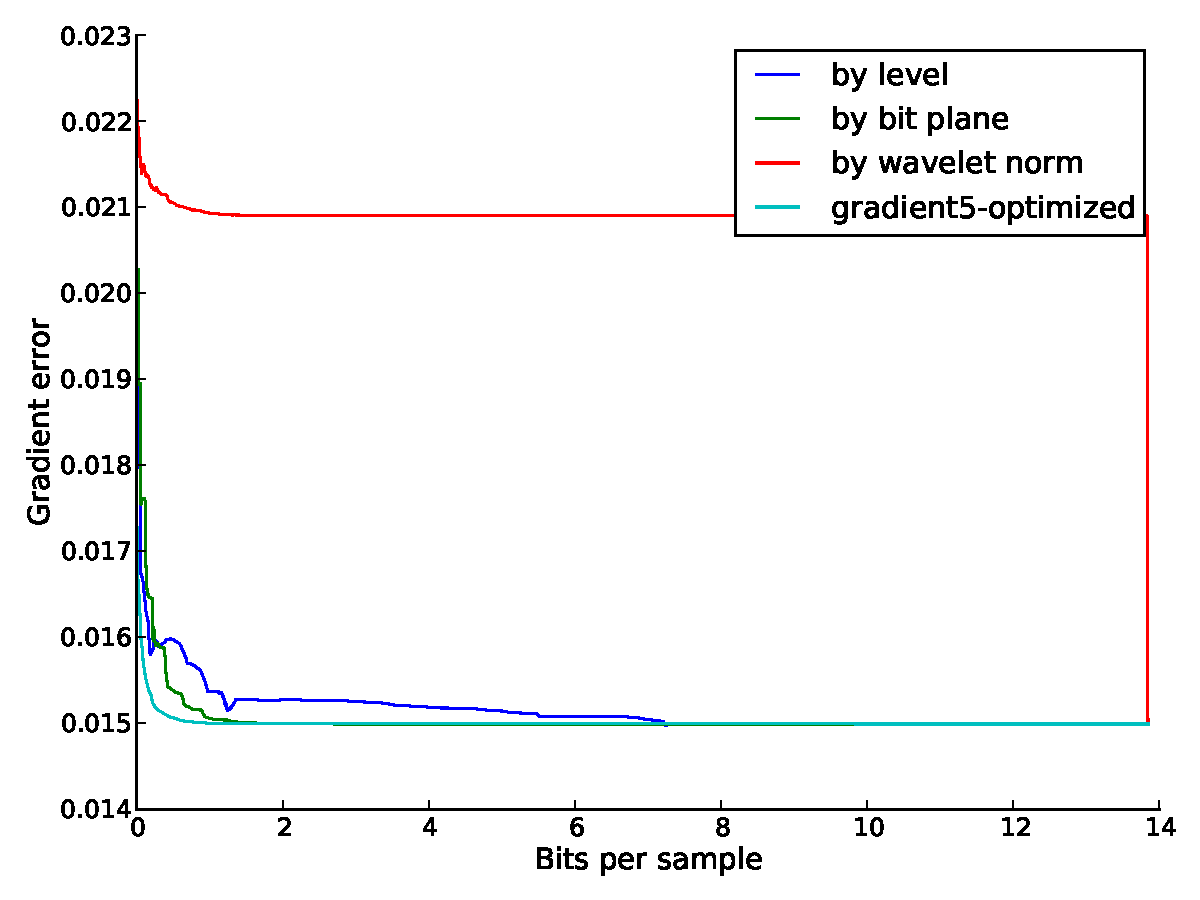
\includegraphics[width=0.48\linewidth]{img/motivation-3d/gradient5-diffusivity.pdf}}
% 	\subcaptionbox{Turbulence}
%  	{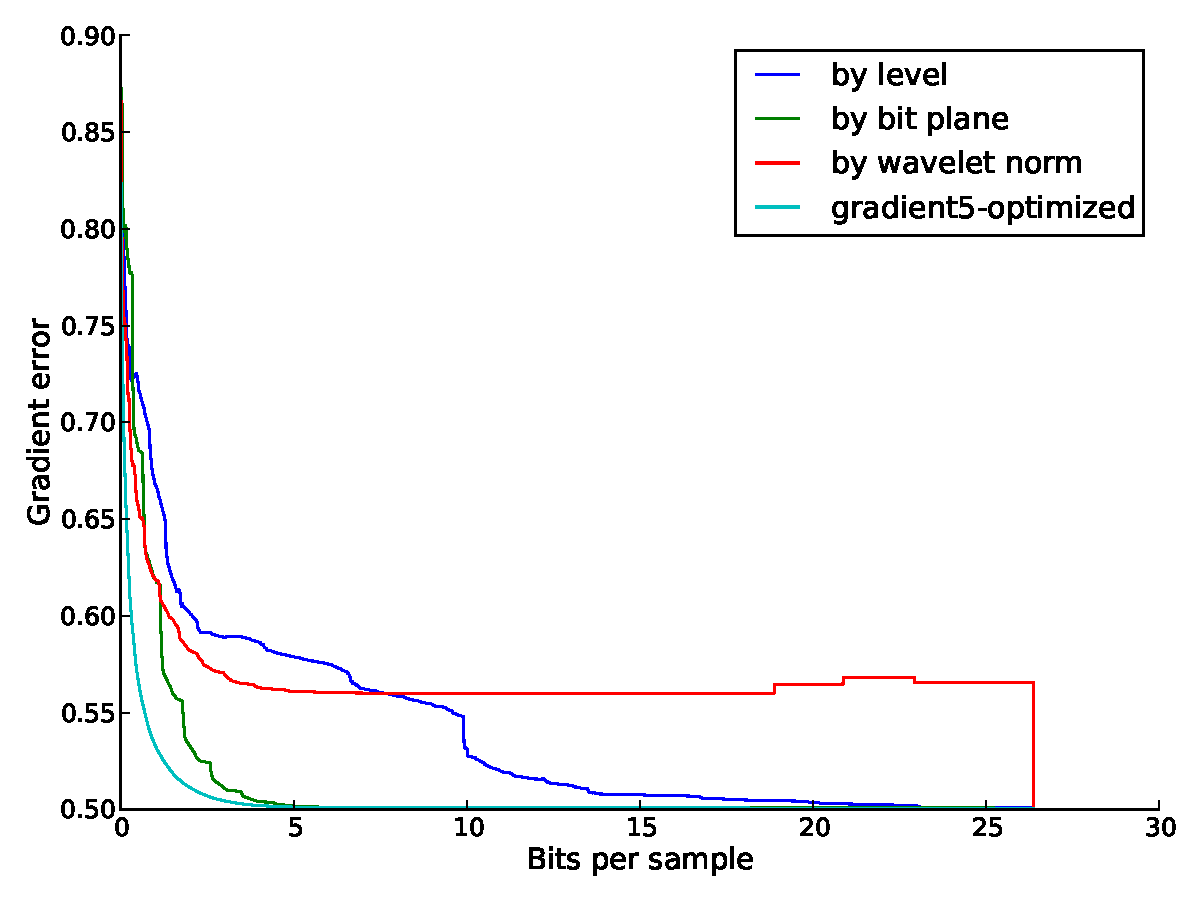
\includegraphics[width=0.48\linewidth]{img/motivation-3d/gradient5-turbulence.pdf}}
% 	\subcaptionbox{Velocity-z}
%  	{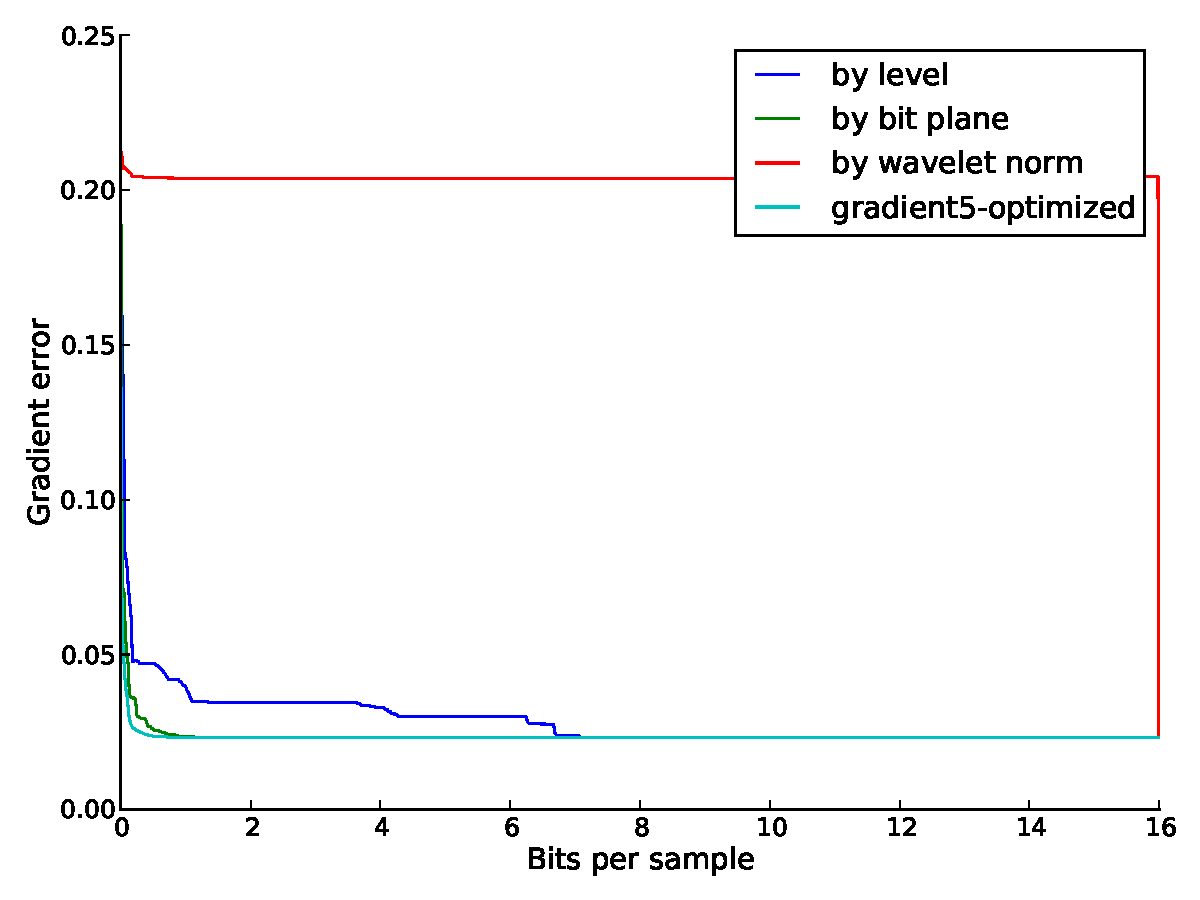
\includegraphics[width=0.48\linewidth]{img/motivation-3d/gradient5-velocityz.pdf}}
%  	\caption{Gradient error (5-point stencil) of reconstructed functions using the three data-agnostic streams
%  	defined in Section \ref{sec:motivation} and the data dependant greedy scheme. Lower is better.
%         The streams are truncated to highlight
%  	the differences, without omitting important information.}
%  	\label{fig:motivation-3d-gradient5}
% \end{figure}

